%!TEX root = ../TTT4150-Summary.tex
\section{Introduction}

%%%%%%%%%%%%%%%%%%%%%%%%%%%%%%%%%%%%%%%%%%%%%%%%%%%%%%%%%%%%
\subsection{A brief history of navigation}

You want to know where you are. Latitude is easy to determine with a sextant, with e.g. the North star or the sun at its highest point. By keeping the home port time with a clock onboard, and measuring time where you are, you can estimate longitude. But clocks (or ``marine chronometers'' if you're a huge nerd) were too inaccurate until John Harrison made a really nice one in the 18th century. Some guys also computed time by observing the moons of Saturn.

%%%%%%%%%%%%%%%%%%%%%%%%%%%%%%%%%%%%%%%%%%%%%%%%%%%%%%%%%%%%
\subsection{Radionavigation}

Ground waves are below HF and hug the terrain. Sky waves are in the same frequency range and reflect back down from the ionosphere. Can communicate past the horizon, but hard to determine propagation time, which is necessary for navigation. Space waves are VHF and up, and go straight.

\subsubsection{Trilateration}
Use propagation time to estimate distance from source. Compute position from several distances. You need three sources for 2D positioning (or two sometimes). For 3D positioning, you need at least one beacon with a large $\Delta h$, which you have with satellites but not ground beacons.

\subsubsection{Hyperbolic positioning}
You get signals from two transmitters, and measure the difference in propagation time. If the difference is zero, your position is equally far from both, and therefore somewhere on a straight line. If the difference is nonzero, your position is a bit closer to one transmitter, and will be along a hyperbolic line. If you have another transmitter pair, each pair gives a line of possible positions, and your location should be at their intersection. Figure \ref{fig:hyperbolic-navigation} illustrates this, with time differences of $0.3$ units between antenna 1 and 2, and $-0.1$ units between 1 and 3. Since you only worry about differences, your clock offset cancels, assuming all transmitter clocks are synced.

\begin{figure}[htbp]
    \centering
    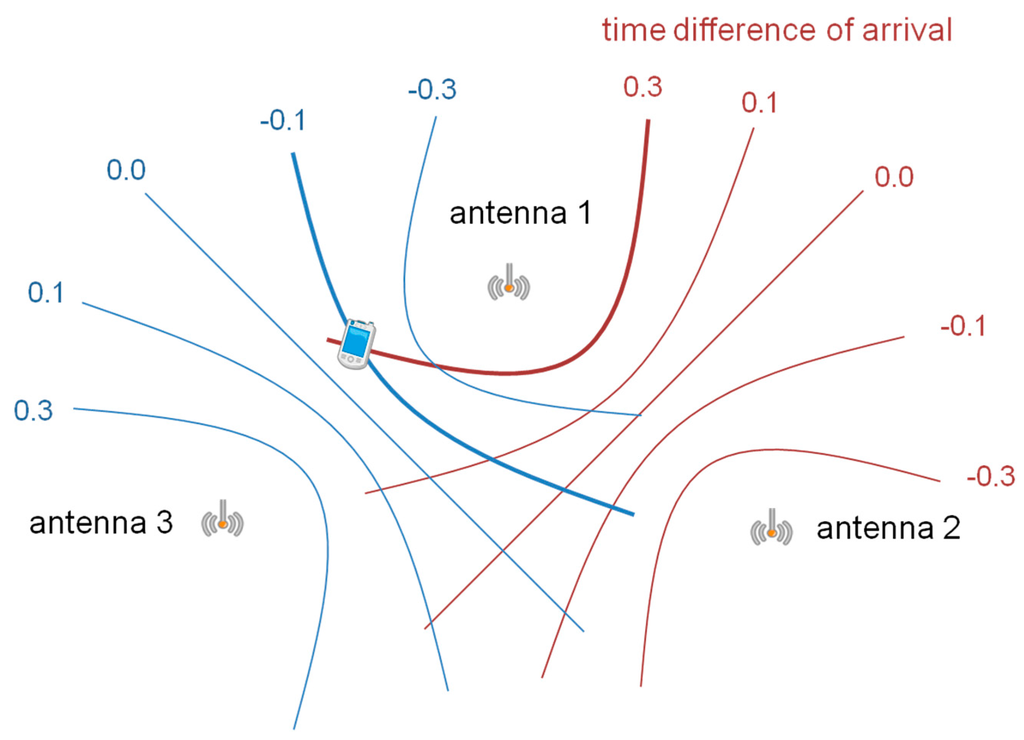
\includegraphics[width=.8\linewidth]{img/hyperbolic-navigation}
    \caption{The principle of hyperbolic navigation}
    \label{fig:hyperbolic-navigation}
\end{figure}

\subsubsection{Doppler positioning}
Observe the doppler shift of a satellite. If you know the orbit, you can determine your position.
